\documentclass{TDP003mall}

\newcommand{\version}{Version 1.7}
\author{Alexander Jonsson, \url{alejo720@student.liu.se}\\
  Joakim Johansson, \url{joajo229@student.liu.se}}
\title{Kravspecifikation}
\date{2016-12-12}
\rhead{Alexander Jonsson \\
Joakim Johansson}

\usepackage{scrextend}
\usepackage{float}

\begin{document}
\projectpage
\section{Revisionshistorik}
\begin{table}[!h]
\begin{tabularx}{\linewidth}{|l|X|l|}
\hline
Ver. & Revisionsbeskrivning & Datum \\\hline
1.7 & Flyttat upp några bör-krav & 2016-12-12 \\\hline
1.6 & Justering och uppflyttning av krav & 2016-11-28 \\\hline
1.5 & Finjustering & 2016-11-24 \\\hline
1.4 & Reviderad utifrån kompletteringsfeedback & 2016-11-23 \\\hline
1.3 & Reviderad utifrån feedback & 2016-11-16 \\\hline
1.2 & Färdig för inlämning till beställargrupp & 2016-11-11 \\\hline
1.1 & Fortsättning på punkterna & 2016-11-09 \\\hline
1.0 & Förstva version, ca hälften av punkterna & 2016-11-08 \\\hline
\end{tabularx}
\end{table}

\newpage

\section{Spelidé}
Tanken med spelet är att två spelare på samma dator ska skjuta projektiler mot varandra. Dessa projektiler kommer antingen färdas högt eller lågt mot spelaren och då måste spelaren ducka respektive hoppa för att undvika projektilen. Om en spelare blir träffad av projektil blir spelaren skadad beroende på projektilens skada. Detta repeteras tills en spelare förlorar allt sitt liv.

\section{Målgrupp}
Målgruppen är två tävlingsinriktade personer som (oftast) känner varandra (helst rivaler). Det är även en bonus om personerna gillar tävlingsinriktade spel med högt tempo.

\section{Spelupplevelse}
Nästan alla människor gillar att vinna, speciellt över sin rival. Det snabba tempot kräver högt fokus vilket ökar adrenalinnivån under matchen samt glädjen när texten “You win!” visas på skärmen. Det snabba tempot och kombinationer av projektiler, banor och karaktärer gör även spelet utmanande.

\newpage

\section{Spelmekanik}
När spelet öppnas visas en huvudmeny där valet “Start Game” och “Exit Game” finns (Kan fyllas på av fler val i framtiden). För att navigera i menyn används upp eller ner piltangenterna samt <enterr> för att välja det markerade alternativet. Vid val av “Start Game” visas en ny skärm där spelarna får välja sin karaktär. Vid val av “Exit Game” stängs spelet av. När båda har valt karaktär kommer spelplanen visas och matchen börja. När en spelare har vunnit och matchen är slut kommer en 'Game Finished'-ruta visas. På denna ruta står det vem som vann och det finns val där spelare 1 får välja att spela igen, byta karaktär eller avsluta spelet. Knappen <escape> kan alltid användas för att gå tillbaka till föregående skärm (dock inte under matchen).
\\ \\
Spelaren kommer kunna vara i tre olika tillstånd; hoppa, ducka eller stående (vanligt). Ända skillnaden mellan dessa tillstånd är om spelaren kommer kunna undvika en projektil eller inte, samt hur karaktären grafiskt ser ut.
\\ \\
Inne på spelplanen kommer spelarna kunna använda tangentbordet för att styra sin karaktär. Nedan är standardknapparna:
\begin{labeling}{right-arrow}
    \item [• Spelare 1:]
    \item [W] Hoppa
    \item [S] Ducka
    \item [A] Gå vänster
    \item [D] Gå höger
    \item [T] Låg projektil
    \item [Y] Hög projektil
    \item []
    \item [• Spelare 2:]
    \item [up-arrow] Hoppa
    \item [down-arrow] Ducka
    \item [left-arrow] Gå vänster
    \item [right-arrow] Gå höger
    \item [.] Låg projektil
    \item [-] Hög projektil
\end{labeling}

\newpage
Spelets flöde ser ut som i denna tabell:
\begin{figure}[H] \label{gameflow}
    \centering
    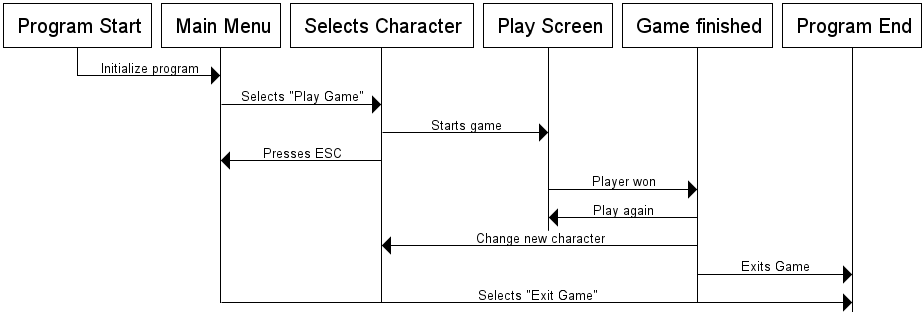
\includegraphics[width = \linewidth]{flow.png}
    \caption{Game Flow}
    \label{fig:Game Flow}
\end{figure}

\newpage

\section{Regler}
\begin{itemize}
\item[] \textbf{Spelplanen:}
\item[] Spelplanen kommer ha två stycken planhalvor.
\item[] Spelplanen kan endast innehålla två spelare.
\item[] Spelaren kan endast röra sig på sin planhalva.
\item[]
\item[] \textbf{Spelaren:}
\item[] Spelaren styr en karaktär som ritas ut på spelplanen.
\item[] Spelaren kan endast röra sig i x-led.
\item[] Spelaren kommer innan spelet välja en karaktär som har olika slags egenskaper.
\item[] Olika karaktärer kommer ha olika hastighet, projektiler och liv.
\item[] Spelare ett och två kommer starta i mitten på vänster respektive höger sida av spelplanen.
\item[] Spelaren kan skjuta projektiler, antingen på hög eller låg nivå.
\item[] Spelarens projektiler kommer skjutas mot motståndarens sida.
\item[] Spelaren kan ducka eller hoppa för att undvika höga respektive låga projektiler.
\item[] Spelaren kommer inte kunna ducka eller hoppa samtidigt som spelaren skjuter en projektil.
\item[] Om spelaren kolliderar med en projektil förlorar spelaren ett liv.
\item[] Om spelaren förlorar alla liv förlorar spelaren och matchen är över.
\item[] 
\item[] \textbf{Projektil:}
\item[] Olika projektiler har olika egenskaper; Hastighet, läge och fördröjning innan projektilen kan skjutas igen.
\item[] Projektilen kan vara i högt eller lågt läge.
\item[] Projektilen kommer försvinna vid kollision.
\end{itemize}

\newpage

\section{Visualisering}
Hur ska spelet se ut? Se \textbf{\ref{fig:Game Flow}} för spelflödet i de olika menyerna.
\subsection{Huvudmeny}
När spelet startas visas en huvudmeny:
\begin{figure}[H]
    \centering
    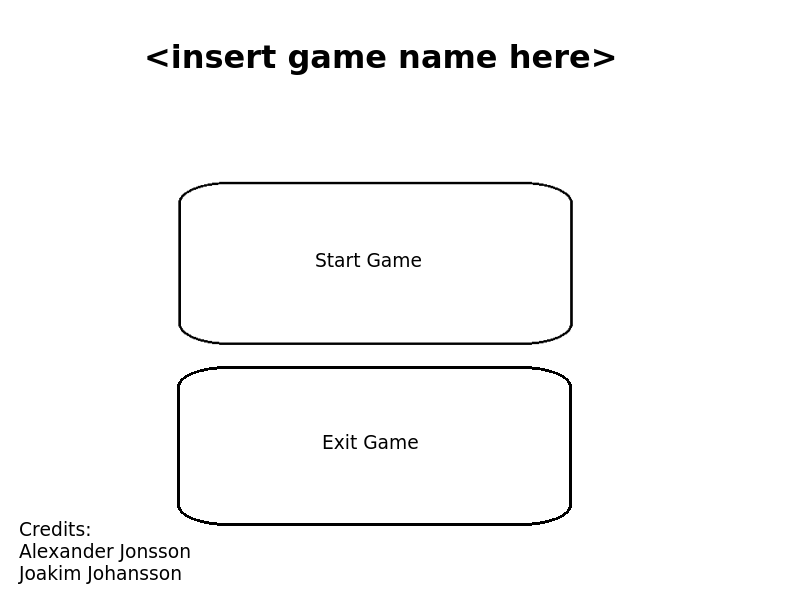
\includegraphics[width = \linewidth]{mainmenu.png}
    \caption{Main menu}
    \label{fig:Main menu}
\end{figure}

\newpage

\subsection{Karaktärväljarrutan}
Vid val av 'Start Game' visas karaktärväljarrutan där spelarna väljer sin karaktär inför matchen:
\begin{figure}[H]
    \centering
    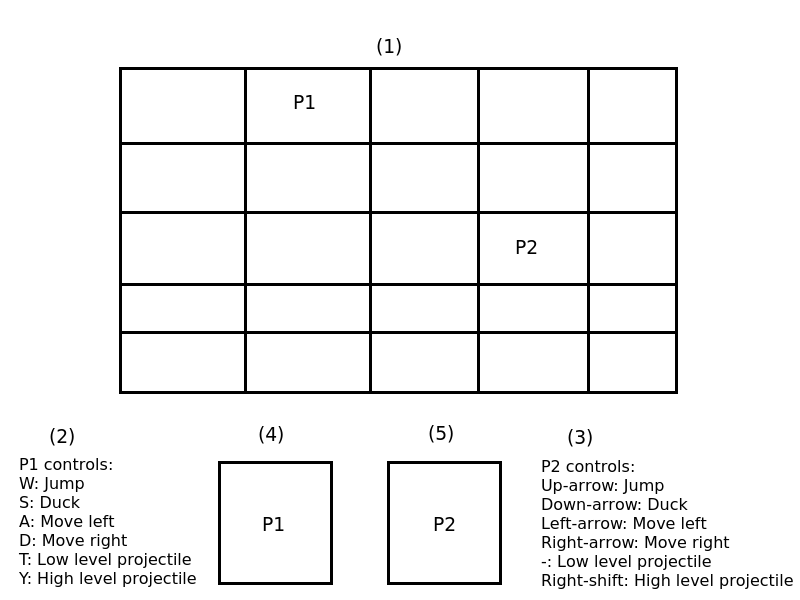
\includegraphics[width = \linewidth]{characterscreen.png}
    \caption{Character screen}
    \label{fig:Character screen}
\end{figure}
\begin{enumerate}
\item Ruta där spelarna får välja karaktär.
\item Spelare etts tangenter.
\item Spelare tvås tangenter.
\item Spelare etts valda karaktär.
\item Spelare tvås valda karaktär.
\end{enumerate}

\subsection{Spelplanen}
\begin{figure}[H]
    \centering
    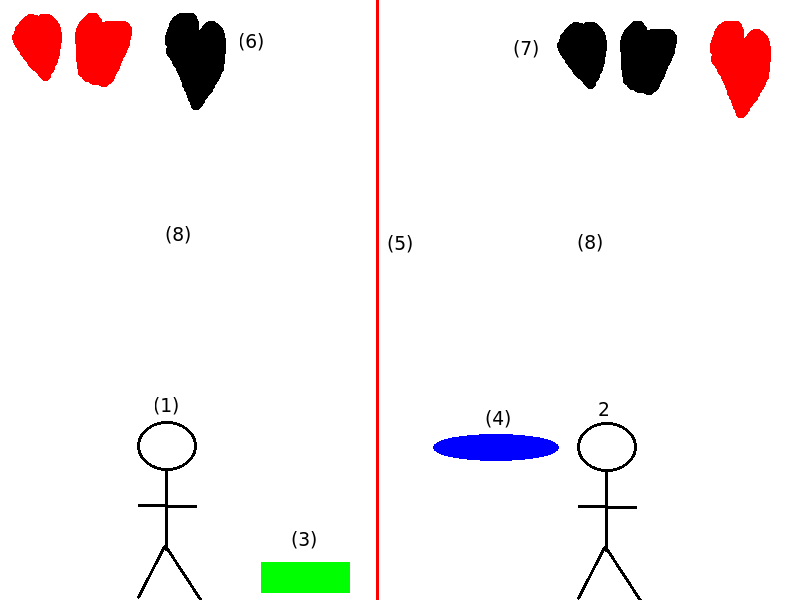
\includegraphics[width = \linewidth]{gameboard.png}
    \caption{Game board}
    \label{fig:Game board}
\end{figure}
\begin{enumerate}
\item Spelare etts karaktär.
\item Spelare tvås karaktär.
\item Exempel på låg projektil.
\item Exempel på hög projektil.
\item Barriär i mitten som grafiskt ska visa att spelarna inte kan gå över till andra sidan.
\item Spelare etts liv.
\item Spelare tvås liv.
\item Bakgrundsbild för att öka spelkänslan.
\end{enumerate}

\subsection{Matchen är slut}
När spelet är slut visas 'Game Finished' rutan. Här står vem som vann och det finns även val för att spela igen, byta karaktärer eller avsluta spelet.
\begin{figure}[H]
    \centering
    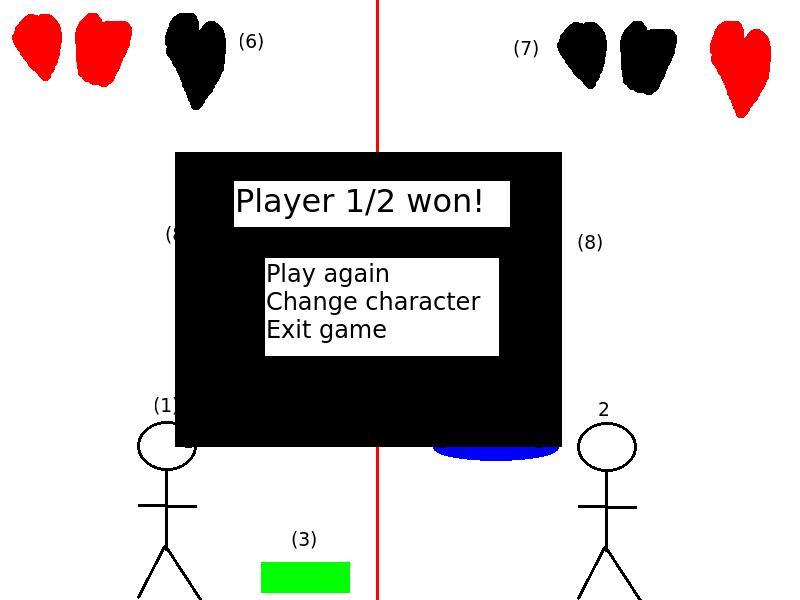
\includegraphics[width = \linewidth]{gamefinished.png}
    \caption{Game board}
    \label{fig:Game board}
\end{figure}

\newpage

\section{Krav}
\begin{enumerate}
\item[] \textbf{Ska-krav}

\item[] 1. Spelplanen ska ha fast storlek och innehålla två planhalvor. En spelare ska inte kunna gå utanför spelplanen eller sin planhalva.
\item[] 2. Spelaren ska styras med tangentbordet och dess standardknappar.
\item[] 3. Spelaren ska endast kunna röra sig i x-led genom att gå vänster eller höger.
\item[] 4. Spelaren ska kunna hoppa och ducka.
\item[] 5. Spelaren ska kunna skjuta projektiler.
\item[] 6. Spelarna ska kunna skjuta en projektil med hög eller låg nivå.
\item[] 9. Spelaren ska alltid vara vänd mot motståndaren.
\item[] 10. Spelare ett och spelare två ska starta i mitten av vänster respektive höger planhalva.
\item[] 18. Olika projektiler ska ha olika egenskaper: Hastighet, läge och fördröjning innan projektilen kan skjutas igen.
\item[] 7. Projektilen ska försvinna vid träff av kant av spelplanen
\item[] 8. Spelet ska kunna spelas mot en annan spelare.
\item[] 11. En projektils riktning ska bero på spelarens riktning.
\item[] 12. Spelaren ska förlora liv vid kollision av en projektil.
\item[] 13. Projektilen ska försvinna vid träff av spelare.
\item[] 14. Spelarna ska kunna undvika höga och låga projektiler genom att ducka respektive hoppa.
\item[] 16. Om spelarens liv blir noll ska spelaren förlora.
\item[] \textbf{Bör-krav}
\item[] 15. Spelaren ska inte kunna skjuta en projektil samtidigt som spelaren hoppar eller duckar.
\item[] 17. Spelaren ska kunna välja en karaktär med olika egenskaper.
\item[] 19. Spelarna ska kunna välja själv vilka knappar som ska användas.
\item[] 20. Det ska finnas olika spelplaner med varierande egenskaper; storlek på planhalvor, bakgrundsbild, namn och spelarens starthöjd.
\item[] 21. Det ska finnas ljudeffekter och musik i spelet.

\end{enumerate}

\newpage

\section{Kravuppfyllelse}
\begin{itemize}
\item Spelet ska simulera en värld som innehåller olika typer av objekt. Objekten ska ha olika beteenden och röra sig i världen och agera på olika sätt när de möter andra objekt.
\item[] \textbf{Uppfylls av kraven 1, 3, 4, 5, 7 ,11, 12, 13, 20}.

\item Det måste finnas minst tre olika typer av objekt och det ska finnas flera instanser av minst två av dessa. T.ex ett spelarobjekt och många instanser av två olika slags fiendeobjekt.
\item[] \textbf{Uppfylls av kraven 1, 5, 6, 8, 18, 20}

\item Ett beteende som måste finnas med är att figurerna ska röra sig över skärmen. Rörelsen kan följa ett mönster och/eller vara slumpmässig. Minst ett objekt, utöver spelaren ska ha någon typ av rörelse. 
\item[] \textbf{Uppfylls av kraven 3, 5, 11}

\item En figur ska styras av spelaren, antingen med tangentbordet eller med musen. Du kan även göra ett spel där man spelar två stycken genom att dela på tangentbordet (varje spelare använder olika tangenter). Då styr man var sin figur. 
\item[] \textbf{Uppfylls av krav 2}

\item Grafiken ska vara tvådimensionell. 
\item[] \textbf{Uppfylls av krav 3, 20}

\item Världen (spelplanen) kan antas vara lika stor som fönstret (du kan göra en större spelplan med scrollning, men det blir lite krångligare). 
\item[] \textbf{Uppfylls av krav 1, 20}

\item Det ska finnas kollisionshantering, det vill säga, det ska hända olika saker när objekten möter varandra, de ska påverka varandra på något sätt. T.ex kan ett av objekten tas bort, eller så kan objekten förvandlas på något sätt, eller så kan ett nytt objekt skapas.
\item[] \textbf{Uppfylls av kraven 7, 12, 13}

\item Spelet måste upplevas som ett sammanhängande spel som går att spela! 
\item[] \textbf{Uppfylls av kraven 1, 2, 3, 5, 7, 8, 11, 12, 13, 14, 15, 16}
\end{itemize}

\end{document}
